\documentclass{article}
    \usepackage[utf8]{inputenc}
    \usepackage[upright]{fourier}
    \usepackage[dvipsnames]{xcolor}
    \usepackage{tikz,tkz-tab}
    \usepackage{amsmath,fullpage}

    \newcommand*{\E}{\ensuremath{\mathrm{e}}}
    \parindent=0pt


\begin{document}

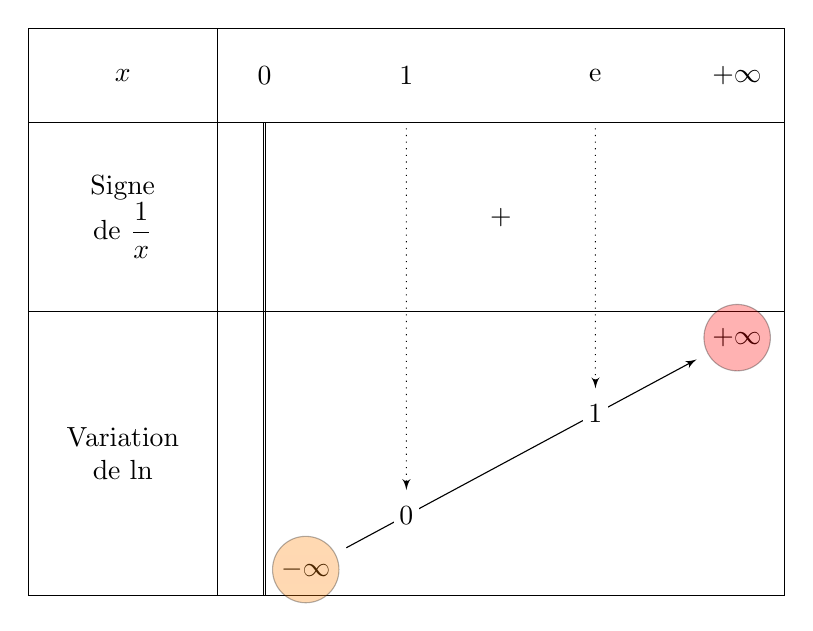
\begin{tikzpicture}[scale=1.2]
    \tkzTabInit[espcl=5]{%
        $x$/1,%
        Signe\\
        de $\dfrac{1}{x}$/2,%
        Variation\\
        de $\ln$/3%
    }{%
        $0$,  $+\infty$%
    }%
    \tkzTabLine {d,+,}%
    \tkzTabVar {D-/ $-\infty$ , + /$+\infty$ }
    \draw[opacity=.3,fill=orange] (FR12) circle (10pt);
    \draw[opacity=.3,fill=red] (FL22) circle (10pt);
    \tkzTabVal[draw] {1}{2} {0.3} {$\text{1}$} {$0$}
    \tkzTabVal[draw] {1}{2} {0.7} {$\E$} {$1$}
\end{tikzpicture}

\end{document}
